\documentclass[onecolumn, draftclsnofoot,10pt, compsoc]{IEEEtran}


\setlength{\parindent}{0em}
\setlength{\parskip}{1em}
\usepackage[margin=0.75in]{geometry}
\geometry{textheight=9.5in, textwidth=7in}
\usepackage{listings}
\usepackage{imakeidx}
\usepackage{graphicx}
\usepackage{float}
\usepackage{listings}
\usepackage{hyperref}
\usepackage{url}
\usepackage{longtable}
\usepackage{enumitem}
\usepackage{setspace}
\singlespacing



\def \DocType{	
	
	Spring Midterm Progress Report	
}


\lstset{
  basicstyle=\small\ttfamily,
 numbers=left,
  numberstyle=\scriptsize,
  showspaces=false,
  showstringspaces=false,
  breaklines=true
}





% 1. Fill in these details
\def \CapstoneTeamName{DSCVL-Overcomers}
\def \CapstoneTeamNumber{69}
\def \GroupMemberTwo{LUCIEN-ARMAND T. TAMNO}
%\def \GroupMemberThree{			}
\def \CapstoneProjectName{Depth sensing with computer vision and lidar}
\def \CapstoneSponsorCompany{}
\def \CapstoneSponsorPerson{ D. Kevin McGrath}


\usepackage{datetime}
\newdate{date}{6}{5}{2018}
\date{\displaydate{date}}

\title{\centering
			
\includegraphics[height=4cm,natwidth=200,natheight=300]{images/osu_logo.png}\\\vspace{.5in}
		\scshape{\huge CS CAPSTONE \DocType \\\vspace{.5in}
		\textbf{\Huge\CapstoneProjectName}\\\vspace{1in}
		\large	\displaydate{date}\\\vspace{.3in}		
			\large {Prepared For}\\\vspace{.1in}
			\textbf{{\Large \CapstoneSponsorPerson}} \\\vspace{.6in}		
				\large {By} \\\vspace{.1in}
				\textbf {Group \CapstoneTeamNumber}\\\vspace{.1in}
				\large {\CapstoneTeamName}\\\vspace{.1in}
				\textbf{ { \GroupMemberTwo}}
}  
}

\IEEEtitleabstractindextext{
 \begin{abstract}
This Depth Sensing with Computer Vision and Lidar report describes the project's goal,presents the current project status towards its final goal, also describes what kinds of problems were encountered during the project development, and finally elaborates on designed solutions  to solve those issues.
 \end{abstract} 
 
}
%%%%%%%%%%%%%%%%%%%%%%%%%%%%%%%%%%%%%%%

\begin{document}
\pagenumbering{gobble}
\maketitle
\IEEEdisplaynontitleabstractindextext
\IEEEpeerreviewmaketitle
\newpage
\pagenumbering{arabic}
\tableofcontents
\newpage
	
\section{Table of Contents}
\tableofcontents
\bibliographystyle{IEEEtran}
\bibliography{ref}


 
\begin{singlespace}
	\section{Definitions}
			\textbf{IR: }\label{def:IR}\par
		IR stands for the infrared technology.

		\textbf{IR Depth Sensor: }\label{def:depthsensor}\par
		A device that calculates distances by emitting infrared signals. 
		
		\textbf{LIDAR: }\label{def:lidar}\par
		Light Detection And Ranging - A method that uses lasers to measure distance
		
		\textbf{Microsoft Kinect: }\label{def:kinect}\par
		A product that uses an IR Depth sensor to measure distances.
		
		\textbf{Logitech Brio Webcam: }\label{def:brio}\cite{logitech}\par
		The webcam model this project shall be using.
		
		\textbf{RPLidar A1: }\label{def:rplidar}[1]\cite{slamtec}\par
		A low-cost LIDAR unit that this project shall be using.
		
		\textbf{RPLidar Solid-state: }\label{def:rplidar2}\cite{leddartech}\par
		A High-cost LIDAR unit single direction with better performances of detecting, measuring and locating liquids and people
	 	
		
		\textbf{Computer Vision: }\label{def:vision}\par
		The methods for acquiring, processing, analyzing, and classifying digital images and extracting information.
		
		
		
		\textbf{Python/C API: }\label{def:API}\cite{Ctype}\par
		API: application programming interface between Python and C programs
		
		\textbf{DSCVL: }\label{def:DSCVL}\par
		Acronym that stands for Depth sensing with computer vision and lidar


		
		
	\section{Project Purpose}
The purpose of the DSCVL\ref{def:DSCVL} project is to come up with an effective solution of painting on a screen an image form a camera with a single point signal from another source technology called Lidar. And for the sake of DSCVL final solution accuracy and better performance,the project concept is to look for any technological tool or system that helps to build an ultimate robust software.

 In fact, on the source technology used in this project, namely the  lidar technology is known to be reliable in outdoor environment in terms of objects distance measurements, and mostly when that lidar technology uses its  16-Segment SOLID-STATE LIDAR equipment also known as the Leddar M16 \ref{def:rplidar2}. One the other hand, a webcam specifically the Logitech Brio Webcam \ref{def:brio} would help to get an image that is located right at the exact same distance than the point signal provided by the new adopted Leddar M16. All this to render with precision the object of interest whether it be a person or a liquid.
 
Moreover, the fact that the lidar technology ( Leddar M16) is much more accurate to provide better objects detection than the IR technology \ref{def:IR} in outdoor, prompts  its de facto adoption in this DSCVL project. However, it is important to know how to use this type of device, how this kind of material would fit into the entire to be built application, and ultimately how to connect the code run by the M16 to other components of the DSCVL project. \par

\section{Current State of the DSCVL}
Though, the past winter term progress report described the RPLidar A1 capability  \ref{def:rplidar} of outputting  useful information but the reality is that the DSCVL project  needed some changes for the sake of better accuracy. some changes took place at different level of the project. And the most important being the replacemnt of RPLiadr A1 by the 16 segment solid state M16 that provides better detection, localization, and distance measurements when is to compares to the RPLidar A1.\par

Additionally, those differences can even be more tangible at the code level, because the M16 model has its code literally written in C program while the RPLidar code is closely related to the python environment. And this M16 factor code-based caused me to conduct researches to figure out how can I make the C program code work in python environment. The result of that research was to discover the python \ref{Ctypes} functionality to play the intermediary role of having the C program code runs in a python environment.With the same idea, I dug a little bit more to finally find out that Visual Studio is the suitable Windows application to implement the python/C API.  

 
\subsection{ Preliminaries and the Python/C API implementation}
	\subsubsection{The default M16-Windows setting}
To stick with the Leddar M16 technology, I have to implement the python/c API\ref{def:API} using the C-code that was shipped with the M16 device. And to do so, I have to make sure first that  the M16 can properly run in a Windows environment by default. And for me to test that functionality, I installed and configured the default M16 settings, as shown in figure \ref{signal} below.

   \begin{figure}[H]
			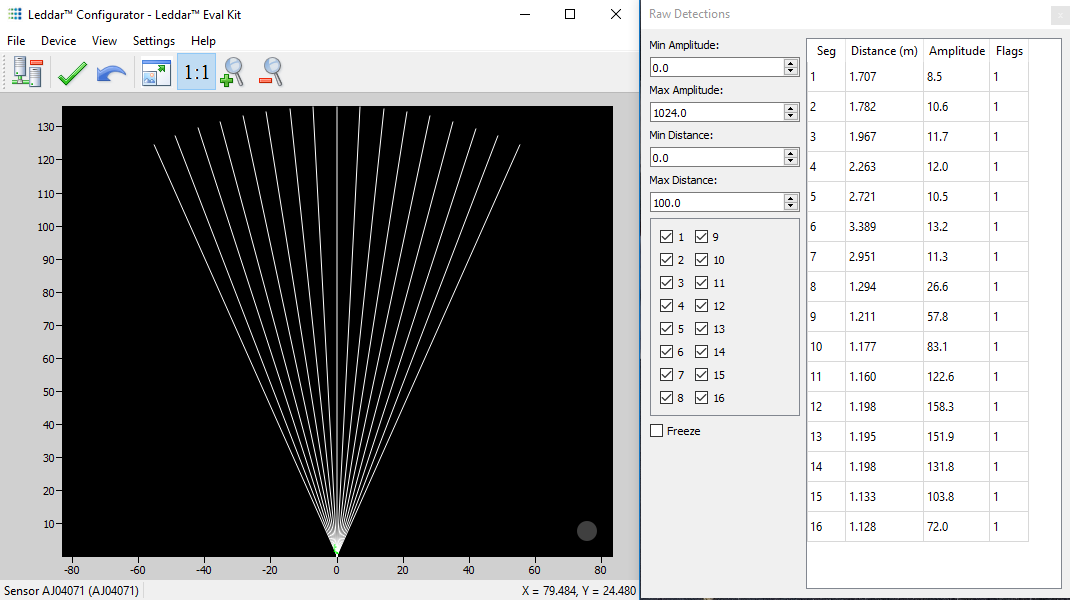
\includegraphics[scale=0.5]{images/signal.PNG}
			\caption{figure}{Leddar M16 outputs distance measurements  using the default windows installation [right] and default M16 screen [left].}
			\label{signal}
		\end{figure}
		
That figure \ref{signal} displays a sample distance outputs as it is supposed to be visualized by a user at the final stage of the DSCVL project. Though, differences may be seen in term of data disposition on the screen,because the M16 code has to run in conjunction with webcam technology to overlay images form the python environment. Hence, the implementation of the DSCVL application has an additional technological constraint to be done via an API.
		
		\subsubsection{ The Python/C API implementation, related issues and attempted solutions}
		
To get the written C language code to python, the Visual studio 2017 application appeared to be the adequate tool to use. Therefore, I installated  visual Studio in Windows 10 system, imported any necessary library to connect the visual Studio  to the Leddar M16 C-code,using the appropriate \cite{Microsoft} documentation related to the topic. 
The remaining bulk of work is  to write and debug the API implementation code to make sure the M16 interacts properly from the visual studio perspective and secondly, to integrate in a single package the python and the M16 C codes, as shown in figure \ref{C-api}.

 \begin{figure}[H]
			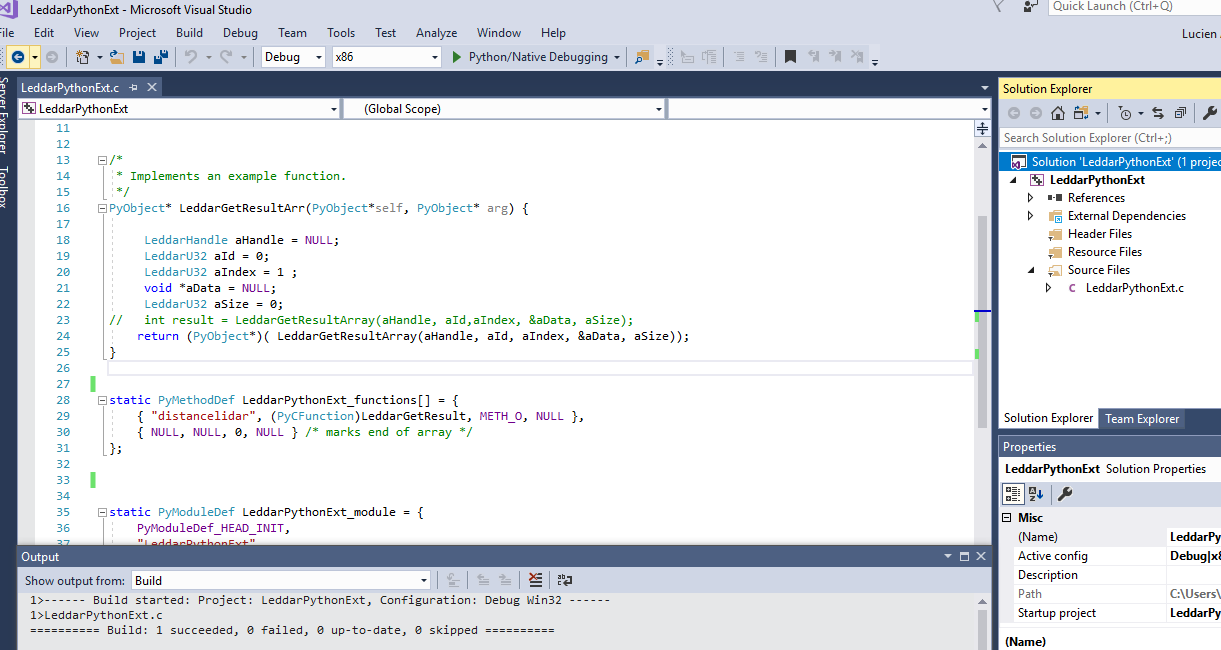
\includegraphics[scale=0.5]{images/C-api.PNG}
			\caption{figure}{Python/C API built in Visual Studio 2017.}
			\label{C-api}
		\end{figure}
		
However, when working on the  above API, I encountered multiple setbacks.among others, the two most important issues are:the slight Leddar M16  differences seen in the the M16 files, for instance I had to change one default header, as shown in figure \ref{change-M16} below.

 \begin{figure}[H]
 \centering
			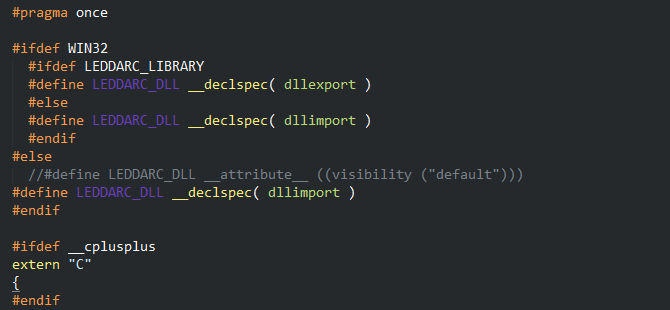
\includegraphics[scale=0.5]{images/change-M16.PNG}
			\caption{figure}{Snippet code changed in the Leddar M16 header file.}
			\label{change-M16}
		\end{figure}

And the worst being found in the current debugging phase that presents a successful result in code checker but generates several linkage errors.  

Finally, I also wrote an additional decorator function in the python module to speed up the python execution module as shown in figure \ref{change-M16}here underneath.

 \begin{figure}[H]
 \centering
			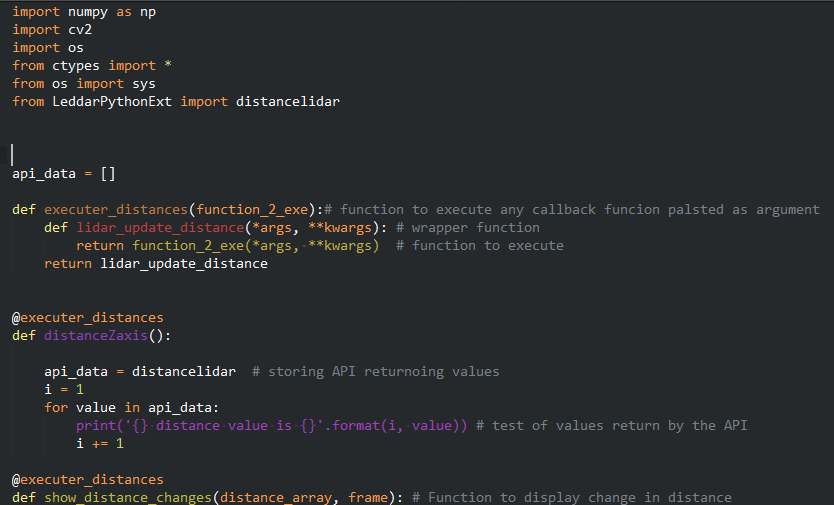
\includegraphics[scale=0.5]{images/python-code.PNG}
			\caption{figure}{Python decorators code.}
			\label{python-code}
		\end{figure}
		
		
\subsection{ Legacy: GUI Interface}

In order to prioritize the DSCVL backend, the Frontend was relegated because the backend is more important and represent the project core functionality as envisioned in the final stage. The GUI downgrade, yet still provides the basic services it has before, but it is not clear whether the final DSCVL system would make use of the legacy graphical user interface.
		
		

	\section{Conclusion}	
	This midterm progress report provides a succinct description of the work done in about a month, presents the focal point of the bulk of work that is to implement the python/C API and ultimate, problems encountered during that implementation process and finally some attempted solutions as remedy to solve those issues. 
		
\end{singlespace}

\end{document}